This section will discuss the implementation, integration and testing of the SafeStreet application. The section aims to prevent any setbacks entailing changes on the project once started its development and do multiple tasks twice. First of all, it is important to divide the project into smaller components in order to have more concrete goals that help keep the developers’ motivation high and make a straightforward development of the project. Therefore, we will divide the project in different components, starting from the ones that are responsible of the basic features and going on until the end, where we will develop the most specific ones. It is not a new method, because it has been studied during this course and it is referred to as ‘bottom-up’ strategy. This method will help providing a better integration of the project tier-by-tier and make different tests of the behaviour of the application before it ends. Going back to our project, we will divide the component related to three main entities, corresponding to USer, Violation and Ticket.
The services that have to be created for each entity are:
User: Sign-UP, Login
Violation: Report Violation, Take Picture, Fill Form, Violation Info, List Vehicles, Street Heatmap, Mine information.
Ticket: Ticket Approval, Statistics, Ticket offenders, Trends.

\begin{sidewaysfigure}
\centering
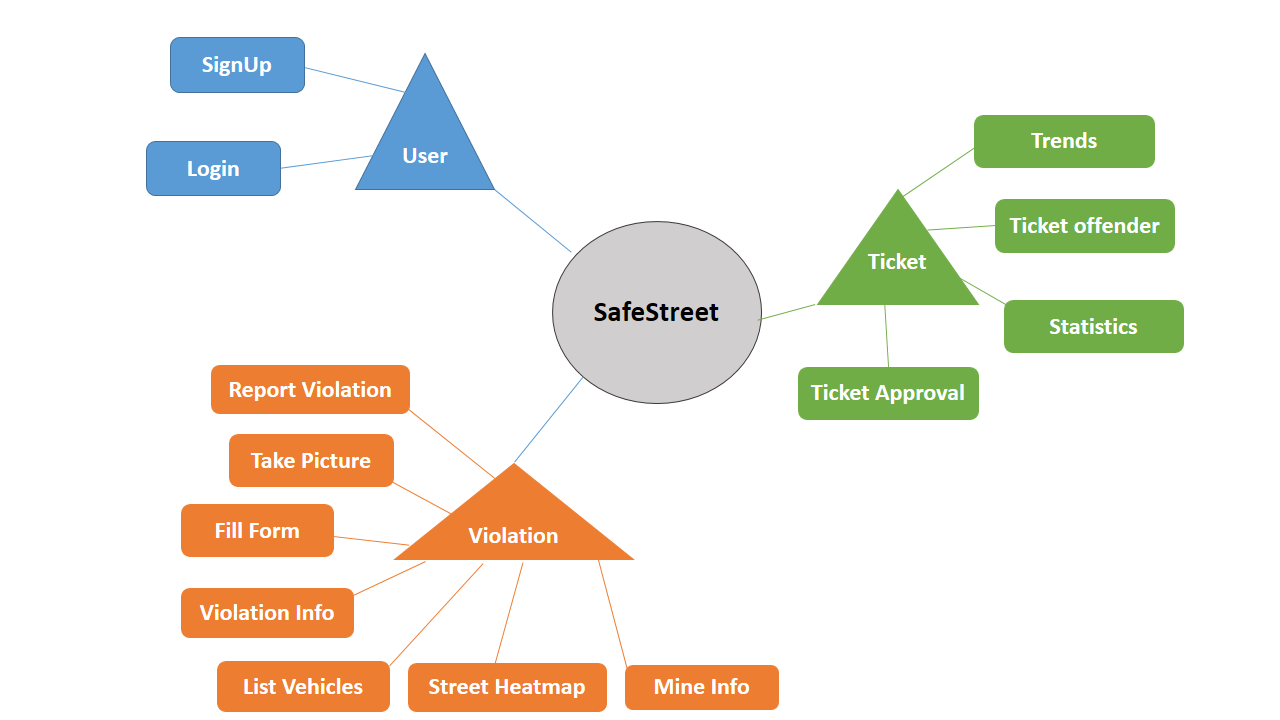
\includegraphics[width=\textwidth]{Images/ImplemetationandTest.png}
\caption{\label{fig:Test} A general overview of the service implementation}
\end{sidewaysfigure}

